\chapter{How to Define a Geometry}
Mice Modules are the objects that control the geometry and fields that are simulated in MAUS. They are used in
conjunction with a datacard file, which provides global run control parameters. Mice Modules are created by reading in
a series of text files when MAUS applications are run.

This geometry information is used primarily by the Simulation application for tracking of particles through magnetic
fields. A few commands are specific to detector Reconstruction and accelerator beam Optics applications.

The Mice Modules are created in a tree structure. Each module is a parent of any number of child modules. Typically the
parent module will describe a physical volume, and child modules will describe physical volumes that sit inside the
parent module. Modules cannot be used to describe volumes that do not sit at least partially inside the volume if the
parent module.

Each Mice Module file consists of a series of lines of text. Firstly the Module name is defined. This is followed by an
opening curly bracket, then the description of the module and the placement of any child modules, and finally a closing
curly bracket. Commands, curly brackets etc must be separated by an end of line character.

Comments are indicated using either two slashes or an exclamation mark. Characters placed after a comment on a line are
ignored.

MAUS operates in a right handed coordinate system $(x,y,z)$. In the absence of any rotation, lengths are
considered to be extent along the \textit{z}{}-axis, widths to be extent along the \textit{x}{}-axis and heights to be
extent along the \textit{y}{}-axis. Rotations $(\theta_{x}, \theta_{y}, \theta_{z})$ are defined
as a rotation about the z-axis through $\theta_{z}$, followed by a rotation about the y-axis through
$\theta_{y}$, followed by a rotation about the x-axis through $\theta_{x}$.

\subsection{Configuration File}
The Configuration file places the top level objects in MICE. The location of the file is controlled by the datacard
\verb|simulation_geometry_file_name|. MAUS looks for the configuration file in the first instance in the directory
\begin{verbatim}
    ${MICEFILES}/Models/Configuration/<MiceModel>
\end{verbatim}
where \verb|${MICEFILES}| is a user-defined environment variable. If MAUS fails to find the file it searches the
local directory.

The world volume is defined in the Configuration file and any children of the world volume are referenced by the
Configuration file. The Configuration file looks like

\begin{verbatim}
    Configuration <Configuration Name>
    {
        Dimensions <x> <y> <z> <Units>
        <Properties>
        <Child Modules>
    }
\end{verbatim}

\verb|<Configuration Name>| is the name of the configuration. Typically the Configuration file
name is given by \verb|<Configuration Name>.dat|. The world volume is always a rectangular box
centred on $(0,0,0)$ with $x$, $y$, and $z$ extent set by the Dimensions. Properties and Child Modules are described below and
added as in any Module.

\subsubsection{Substitutions}
It is possible to make keyword substitutions that substitutes all instances of \verb|<name>| with
\verb|<value>| in all Modules. The syntax is

\begin{verbatim}
    Substitution <name> <value>
\end{verbatim}

\verb|<name>| must start with a single \$ sign. Substitutions must be defined in the Configuration file.
Note this is a direct text substitution in the MiceModules before the modules are parsed properly. So for example,

\begin{verbatim}
    Substitution $Sub SomeText
    PropertyString FieldType \$Sub}
    PropertyDouble \$SubValue 10}
\end{verbatim}

would be parsed as MAUS like

\begin{verbatim}
    PropertyString FieldType SomeText}
    PropertyDouble SomeTextValue 10}
\end{verbatim}

\subsubsection{Expressions}
The use of equations in properties of type double and Hep3Vector is also allowed in place of a single value. So, for
example, 
\begin{verbatim}
    PropertyDouble FieldStrength 0.5*2 T
\end{verbatim}
would result in a FieldStrength property of 1 Tesla.\texttt{ }

\subsubsection{Expression Substitutions}
Some additional variables can be defined in specific cases by MAUS itself for substitution into experssions, in which
case they will start with @ symbol. For these variable substitutions, it is only possible to make the substitution into
expressions. So for example,
\begin{verbatim}
    PropertyDouble ScaleFactor 2*@RepeatNumber
\end{verbatim}
Would substitute @RepeatNumber \ into the expression. @RepeatNumber \ is defined by MAUS when repeating modules are
used (see RepeatModule2, below). Note the following code is not valid
\begin{verbatim}
    PropertyString FileName File@RepeatNumber //NOT VALID
\end{verbatim}
This is because Expression Substitutions can only be used in an expression (i.e. an equation).

\subsection[Module Files]{Module Files}
Children of the top level Mice Module are defined by Modules. MAUS will attempt to find a module in an external file.
The location of the file is controlled by the parent Module. Initially MAUS looks in the directory
\begin{verbatim}
    ${MICEFILES}/Models/Modules/<Module>
\end{verbatim}
If the Mice Module cannot be found, MAUS searches the local directory. If the module file still cannot be found,
MAUS will issue a warning and proceed.

The Module description is similar in structure to the Configuration file:
\begin{verbatim}
    Module <Module Name>
    {
        PropertyString Volume  <Volume Type>
        PropertyHep3Vector Dimensions  <Dimension1> <Dimension2> <Dimension3> <Units>
        <Properties>

        <Child Modules>
    }
\end{verbatim}
\verb|<Module Name>| is the name of the module. Typically the Module file name is given by
\verb|<Module Name>.dat|.

The definition of Volume, Dimensions, Properties and Child Modules are described below.

\subsection{Volume and Dimensions}
The volume described by the MiceModule can be one of several types. Replace \verb|<Volume Type>| with the
appropriate volume below. Cylinder, Box and Tube define cylindrical and cuboidal volumes.
Polycone defines an arbitrary volume of rotation and is described in detail below. Wedge describes a wedge with a
triangular projection in the y-z plane and rectangular projections in x-z and x-y planes. Quadrupole defines an
aperture with four cylindrical pole tips.

In general, the physical volumes that scrape the beam are defined independently of the field maps. This is the more
versatile way to do things, but there are some pitfalls which such an implementation introduces. For example, in
hard-edged fields like pillboxes, tracking errors can be introduced when MAUS steps into the field region. This can
be avoided by adding windows (probably made of vacuum material) to force GEANT4 to stop tracking, make a small step
over the field boundary, and then restart tracking inside the field. However, such details are left for the user to
implement.

\begin{center}
\tablefirsthead{\hline
{\bfseries Volume} &
\multicolumn{1}{m{4.321cm}|}{{\bfseries Dimension1}} &
\multicolumn{1}{m{4.564cm}|}{{\bfseries Dimension2}} &
{\bfseries Dimension3}\\}
\tablehead{\hline
{\bfseries Volume} &
\multicolumn{1}{m{4.321cm}|}{{\bfseries Dimension1}} &
\multicolumn{1}{m{4.564cm}|}{{\bfseries Dimension2}} &
{\bfseries Dimension3}\\}
\tabletail{}
\tablelasttail{}
\begin{supertabular}{|m{2.659cm}|m{4.321cm}m{4.564cm}m{5.25cm}|}
\hline
None &
\multicolumn{3}{m{14.535cm}|}{No dimensions required. Note cannot define daughter Modules for this volume type.}\\\hline
Cylinder &
\multicolumn{1}{m{4.321cm}|}{Radius} &
\multicolumn{1}{m{4.564cm}|}{Length in z} &
Not used (leave blank)\\\hline
Box &
\multicolumn{1}{m{4.321cm}|}{Width in x} &
\multicolumn{1}{m{4.564cm}|}{Height in y} &
Length along z\\\hline
Tube &
\multicolumn{1}{m{4.321cm}|}{Inner Radius} &
\multicolumn{1}{m{4.564cm}|}{Outer Radius} &
Length in z\\\hline
Trapezoid &
\multicolumn{1}{m{4.321cm}|}{Half Width in x} &
\multicolumn{1}{m{4.564cm}|}{Half Height in y} &
Half Length in z\\\hline
Wedge &
\multicolumn{3}{m{14.535cm}|}{See documentation below.}\\\hline
Polycone &
\multicolumn{3}{m{14.535cm}|}{No dimensions required. Volume defined from external file.}\\\hline
Quadrupole &
\multicolumn{3}{m{14.535cm}|}{No dimensions required. Dimensions defined from module properties.}\\\hline
Multipole &
\multicolumn{3}{m{14.535cm}|}{No dimensions required. Dimensions defined from module properties.}\\\hline
Boolean &
\multicolumn{3}{m{14.535cm}|}{No dimensions required. Dimensions defined from module properties.}\\\hline
Sphere &
\multicolumn{3}{m{14.535cm}|}{See documentation below.}\\\hline
\end{supertabular}
\end{center}

\subsection{Properties}
Many of the features of MAUS that can be enabled in a module are described using properties. For example, properties
enable the user to define detectors and fields. Properties can be either of several types: PropertyDouble,
PropertyString, PropertyBool, PropertyHep3Vector or PropertyInt. A property is declared via
\begin{verbatim}
    <Property Type> <Property Name> <Value> <Units if appropriate>
\end{verbatim}
Different properties that can be enabled for Mice Modules are described elsewhere in this document. Properties of type
PropertyDouble and PropertyHep3Vector can have units. Units are defined in the CLHEP library. Units are case sensitive;
MAUS will return an error message if it fails to parse units. Combinations of units such as T/m or N*m can be defined
using '*' and '/' as appropriate. Properties cannot be defined more than once within the same module.

\subsection{Child Modules}
Child Modules are defined with a position, rotation and scale factor. This places, and rotates, the child volume and any
fields present relative to the parent volume. Scale factor scales fields defined in the child module and any of its
children. Scale factors are recursively multiplicative; that is the field generated by a child module will be scaled by
the product of the scale factor defined in the parent module and all of its parents.

The child module definition looks like:
\begin{verbatim}
    Module <Module File Name>
    {
        PropertyHep3Vector Position  <x position> <y position> <z position> <Units>
        PropertyHep3Vector Rotation  <x rotation> <y rotation> <z rotation> <Units>
        PropertyDouble ScaleFactor <Value>
        <Define volume, dimensions and properties for this instance only>
    }
\end{verbatim}
MAUS searches for \verb|<Module File Name>| first relative to \verb|${MICEFILES}/Models/Modules/| and subsequently
relative to the current working directory. The position and rotation default to $0, 0, 0$ and the \verb|scale factor| defaults
to $1$.

\liststyleLi
\begin{itemize}
\item Volume, Dimension and Properties of the child module can be defined at the level of the parent; in this case these
values will be used only for this instance of the module.
\end{itemize}
\liststyleLii
\begin{itemize}
\item If no file can be found, MAUS will press on regardless, attempting to build a geometry using the information
defined in the parent volume.
\end{itemize}
\subsection[Module Hierarchy and GEANT4 Physical Volumes]{Module Hierarchy and GEANT4 Physical Volumes}
\begin{figure}[!htb]
\begin{center}
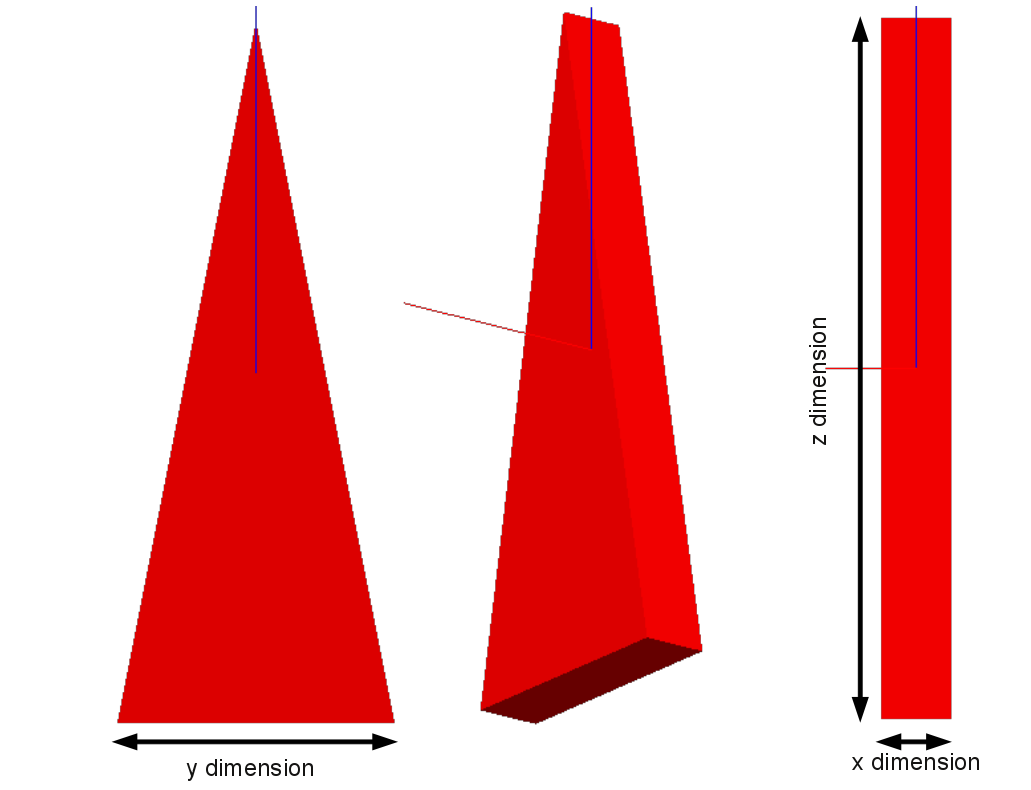
\includegraphics[width=0.5\textwidth]{mice_modules/volume_hierarchy.png}
\caption{The diagram shows a schematic for a square placed inside a cylinder inside a rectangle. This nesting must be replicated
         in the MiceModules in order for the volumes to be correctly represented by MAUS.}
\end{center}
\end{figure}
MAUS enables users to place arbitrary physical volumes in a GEANT4 geometry. The
formatting of MAUS is such that users are encouraged to use the GEANT4 tree structure for placing physical volumes.
This is a double-edged sword, in that it provides users with a convenient interface for building geometries, but it is
not a terribly safe interface.

Consider the cartoon of physical volumes shown above. Here there is a blue volume sitting inside a red volume sitting
inside the black world volume. For the volumes to be represented properly, the module that represents the blue volume
MUST be a child of the module that represents the red volume. The module that represents the red volume MUST, in turn,
be a child of the module that represents the black volume, in this case the Configuration file.

What would happen if we placed the blue volume directly into the Black volume, i.e. the Configuration file? GEANT4 would
silently ignore the blue volume, or the red volume, depending on the order in which they are added into the GEANT4
geometry. What would happen if we placed the blue volume overlapping the red and black volumes? The behaviour of GEANT4
is not clear in this case.

\liststyleLiii
\begin{itemize}
\item Never allow a volume to overlap any part of another volume that is not it's direct parent.
\end{itemize}
It is possible to check for overlaps by setting the datacard \textit{CheckVolumeOverlaps} to 1.

\subsection{A Sample Configuration File}
Below is listed a sample configuration file, which is likely to be included in the file
\textit{ExampleConfiguration.dat;} the actual name is specified by the datacard MiceModel.
\begin{verbatim}
    Configuration ExampleConfiguration
    {
        Dimensions 1500.0 1000.0 5000.0 cm
        PropertyString Material AIR
        Substitution $MyRedColour 0.75
        Module BeamLine/SolMag.dat
        {
            Position 140.0 0.0 -2175.0 cm
            Rotation 0.0 30.0 0.0 degree
            ScaleFactor 1.
        }
        Module BeamLine/BendMag.dat
        {
            Position 0.0 0.0 -1935.0 cm
            Rotation 0.0 15.0 0.0 degree
            ScaleFactor 1.
        }
        Module NoFile_Box1
        {
            Volume Box
            Dimension 1.0 1.0 1.0
            Position 0.0 0.0 200.0 cm
            Rotation 0.0 15.0 0.0 degree
            PropertyString Material  Galactic
            PropertyDouble RedColour $MyRedColour
        }
        Module NoFile_Box2}
        {
            Volume Box
            Dimension 0.5 0.5 0.5*3 m //z length = 0.5*3 = 1.5 m
            Rotation  0.0 15.0 0.0 degree //Rotation relative to parent
            PropertyString Material  Galactic
            PropertyDouble RedColour $MyRedColour
        }
    }
\end{verbatim}

\subsection{A Sample Child Module File}
Below is listed a sample module file, which is likely to be included in the file \textit{SolMag.dat}; the actual
location is specified by the module or configuration that calls FCoil. The module contains a number of properties that
define the field.

\begin{verbatim}
    Module SolMag
    {
        Volume Tube
        Dimensions 263.0 347.0 210.0 mm
        PropertyString Material Al
        PropertyDouble BlueColour 0.75
        PropertyDouble GreenColour 0.75
        //field}
        PropertyString FieldType      Solenoid
        PropertyString FileName       focus.dat
        PropertyDouble CurrentDensity 1.
        PropertyDouble Length         210. mm
        PropertyDouble Thickness      84. mm
        PropertyDouble InnerRadius    263. mm
    }
\end{verbatim}

